% ==============================================
% Packaging Technology options and theory
% ==============================================

\section{Packaging Technology Options}

\begin{itemize}
	\item Flip Chip
	\begin{itemize}
		\item Solder balls on Nickel/Gold finish (time consuming) % time consuming in regards to time added to fabrication
		\item Heat Spreader (Graphene-based)
		\item Underfill materials
		\item Redistribution layers(?)
	\end{itemize}
	\item Copper Pillar (flipped die)
	\begin{itemize}
		\item 30 \unit{\micro \metre} min diameter, better thermal conductivity
		\item More stable (no need for underfill)
		\item Heat spreader most likely needed
	\end{itemize}
	\item Chip on board
	\begin{itemize}
		\item Glue chip on PCB cavity (non-conductive glue needed if BSE)
		\item Only backside cooling available
		\item Connect with wirebonds
	\end{itemize}
	\item Open cavity QFN
	\begin{itemize}
		\item Similar to chip on board
		\item Extra penalty due to higher thermal resistance of package
	\end{itemize}
\end{itemize}

On packaging from Elad:

\begin{info}
	I was asked to give my opinion regarding silicone component packaging.\\
	Since the size of the component is (on the major axis) 3.5 and down bonds to the ground are required on both sides, you need to verify the distance of the pads of the component from the edge of the die, the closer you can use a smaller ground surface. Assuming that the pads reach the edge, it will be possible to use a ground surface in a package of  4.1 \unit{mm}, depending on the planning design rules of the Assembly house. \\
	In light of this, I recommend considering using the RJR air cavity 6 x 6 \unit{mm} package and its lid. \\
	Regarding the glue, since the CTE gap between the component and the packaging is large, I recommend using the glue (I think they thought of this direction) me8456lv, which has a thermal conductivity of around 6W/m \\
	\href{https://www.rjrtechnologies.com/}{\textbf{rjrtechnologies website}}
\end{info}

QFN stands for \textbf{Q}uad \textbf{F}lat \textbf{N}o lead.

Number of pins is important for packaging - keep it below 32.

% List of my questions for me?
% Is this open cavity? What are cavities used for?
% What about the extra penalty due to higher thermal resistance (thermal conductivity)
% What is laminate?


\begin{figure}[ht!]
	\centering % try to centre it
	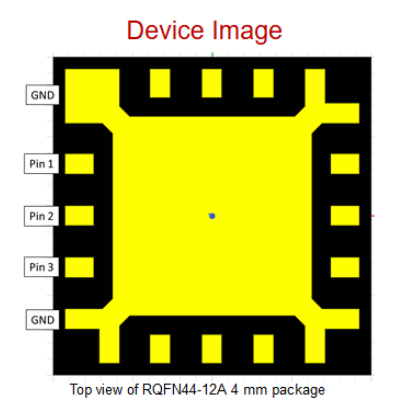
\includegraphics[width=0.5\linewidth]{Figures/RQFN-4-mm.png}
	\caption{RQFN packaging example }
	\label{fig:rqfn-example}
\end{figure}

\subsection{Flip Chip as a packaging option}

Flip chip, also known as controlled collapse chip connection or its abbreviation, C4, is a method for interconnecting dies such as semiconductor devices, IC chips, integrated passive devices and microelectromechanical systems (MEMS), to external circuitry with solder bumps that have been deposited onto the chip pads. This is in contrast to wire bonding, in which the chip is mounted upright and fine wires are welded onto the chip pads and lead frame contacts to interconnect the chip pads to external circuitry.

% ==============================================
% PACKAGING House options
% ==============================================

\subsection{Packaging house options}

Packaging house options are:

\begin{itemize}
	\item TAI PRO
	\begin{itemize}
		\item \href{https://www.taipro.be/production}{\textbf{Website for Production}}
	\end{itemize}
	\item PacTech (IHP has collaboration with them)
	\begin{itemize}
		\item \href{https://pactech.com/wafer-level-packaging-services/}{\textbf{Website for Wafer Level Packaging Services}}
	\end{itemize}
	\item IZM
	\begin{itemize}
		\item \href{https://www.izm.fraunhofer.de/en/abteilungen/wafer-level-system-integration/leistungsangebot/fine-pitch-bumping-for-pixel-detectors.html}{\textbf{Website for Fine Pitch Bumping for Pixel Detectors}}
		\item \href{https://www.izm.fraunhofer.de/en/abteilungen/wafer-level-system-integration/leistungsangebot/single_chip_bumping.html}{\textbf{Website for Single Chip Bumping}}
	\end{itemize}
	\item RJR Technologies
	\begin{itemize}
		\item \href{https://www.rjrtechnologies.com/}{\textbf{Website}}
	\end{itemize}
\end{itemize}

% Additional option is GP technologies

% Belgium company is for packaging

% California houses
% QP technologies
% spectrum semi

\subsection{Packaging terms by AMPLEON}

Packaging is an important element in RF power transistors, influencing both the cost-efficiency and performance of a given device. Since peak powers can vary widely, from as low as 5 W to more than 1 kW, a range of packages is needed to cover every application. The choice of package format (air-cavity or overmolded plastic), often depends on the design requirements, and any \textbf{trade-offs to be made between performance and cost.} \\

\href{https://www.ampleon.com/packages.html}{\textbf{Source for ampleon packaging}}

Types of packaging:

\begin{itemize}
	\item Air-Cavity Ceramic (ACC)
	\item Air-Cavity Plastic (ACP)
	\item Overmolded Plastic (OMP)
\end{itemize}

\subsection{Definition of terms regarding packaging from RJR technologies}

\begin{itemize}
	\item PRQFN - stands for RJR's thermally enhanced \textbf{P}ower ai\textbf{R}-cavity \textbf{Q}uad \textbf{F}lat \textbf{N}o-leads package
	\item Substrate - the base material that holds the circuit and components (chips, wires, and caps) of semiconductor devices
	\item Coupon - a square panel containing a cluster of substrates
	\item Strip - a rectangular laminate panel containing 4 in-line coupons
	\item Laminate - a substrate technology composed of several layers that are pressed/laminated together
	\item Heatslug - a square or rectangular Cu-coin inserted in the middle of the laminate substrate
	\item Via hole - a hole drilled from top to bottom of the substrate and is used for connecting the terminals on top to the corresponding soldering pads underneath
	\item ENEPIG - stands for Electroless Nickel Electroless Palladium Immersion Gold; the die bondable and wire bondable plating on top of Cu-traces in a laminate
	\item Terminal - metal (Cu) traces that serves as connection of the device into the outside world
	\item Solder resist - a thin layer of polymer that is usually applied on top of Cu-traces of the laminate substrate for protection against oxidation, and around the soldering pads to prevent solder bridges from forming between closely spaced solder pads
\end{itemize}

\subsection{Die layout example}

This is an example (estimation) for this PLL project die size and layout:

\begin{figure}[ht!]
	\centering % try to center it
	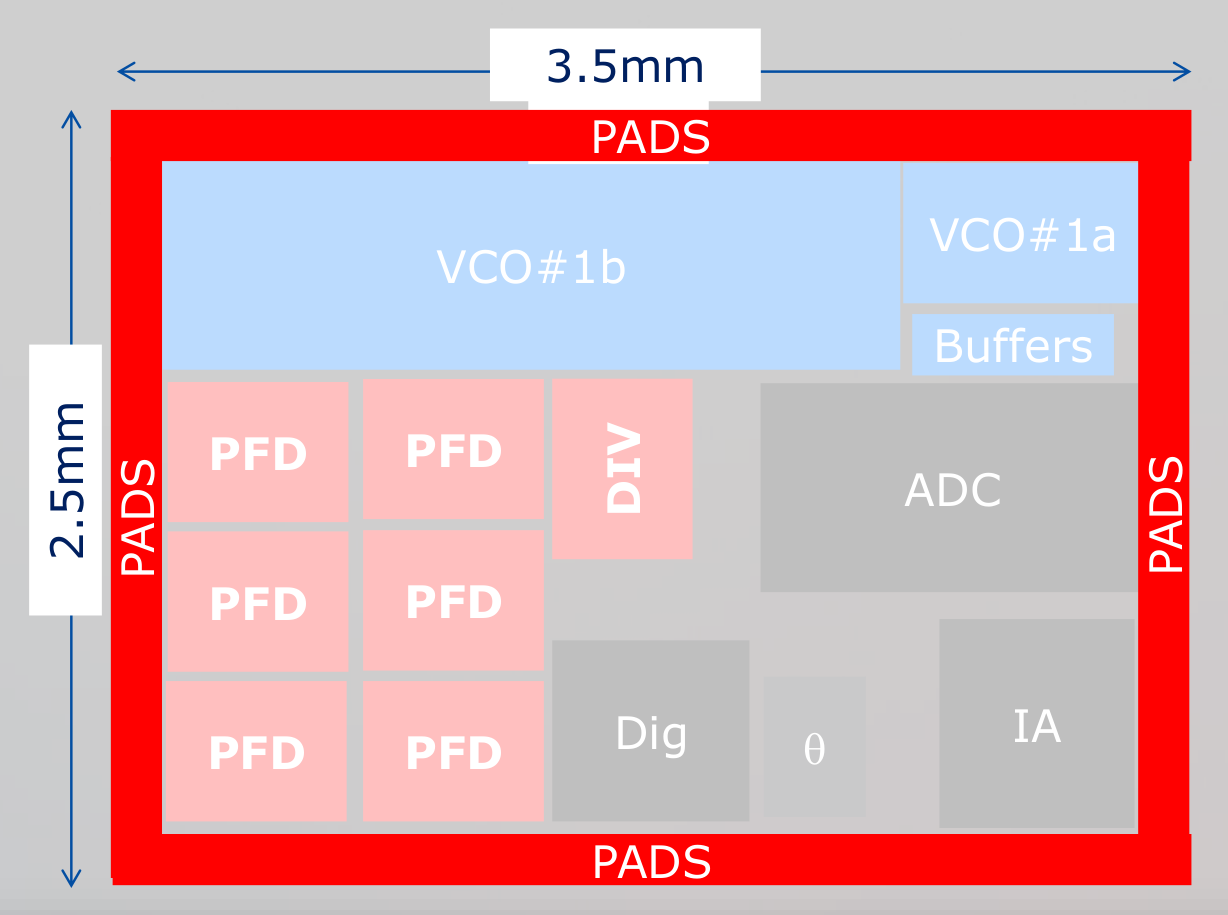
\includegraphics[width=0.5\linewidth]{Figures/die-size-with-pads.png}
	\caption{Die layout with pads }
	\label{fig:die-size-with-pads}
\end{figure}

Also important is the pin count. Absolute minimum is 8 \unit{\milli\metre} x 8 mm.

\begin{figure}[ht!]
	\centering % try to center it
	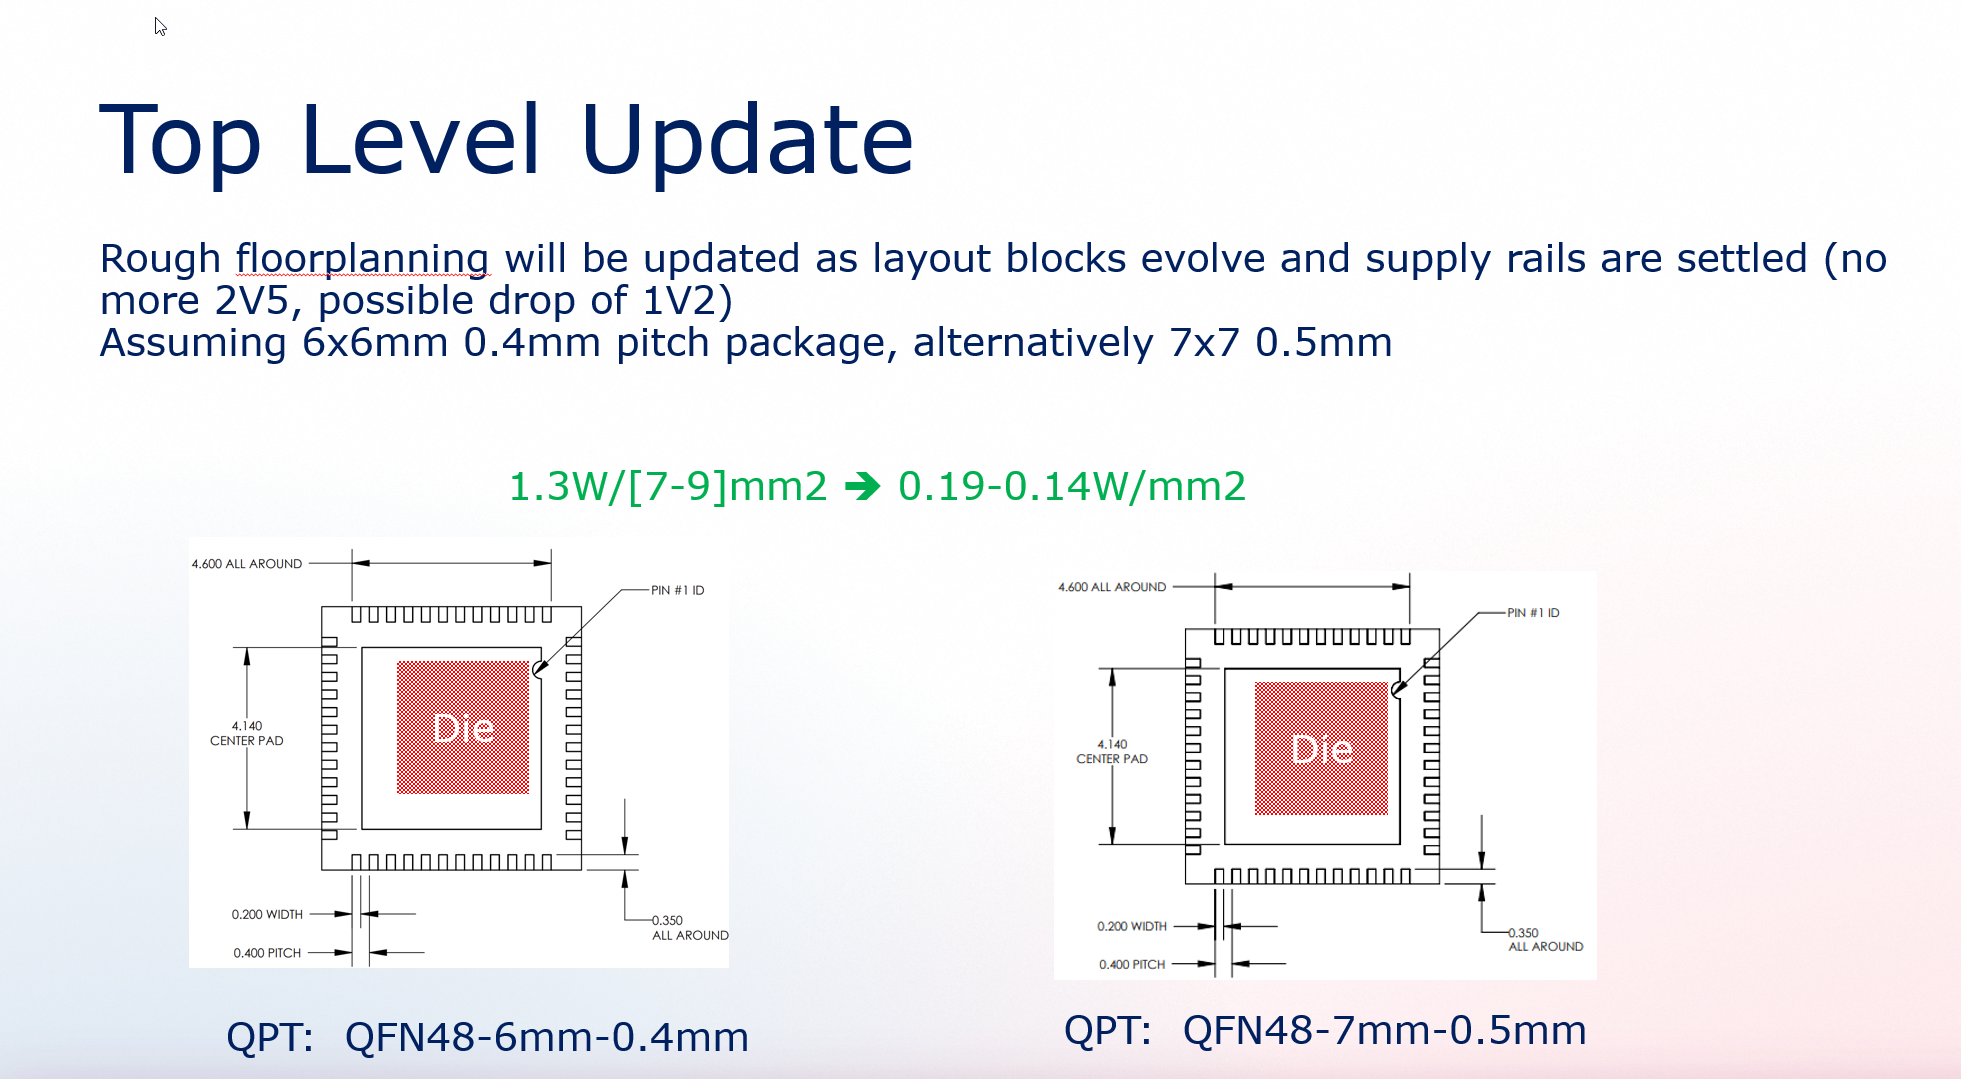
\includegraphics[width=0.5\linewidth]{Figures/powerpoint-toplevel-packaging.png}
	\caption{Top layout and packaging choice}
	\label{fig:powerpoint-toplevel-packaging}
\end{figure}